% A reference card for the darktable photography workflow application.
% Copyright (C) 2015 Mark Richters

\RequirePackage[l2tabu,orthodox]{nag}
\documentclass[\ArgLang,\ArgFormat,9pt]{extarticle}
\usepackage[utf8]{inputenc}
\usepackage[T1]{fontenc}
\usepackage{babel}
\usepackage{textcomp}
%\usepackage{helvet}
\usepackage{newcent}
\usepackage[landscape,margin={7mm,20mm}]{geometry}
\usepackage{microtype}
\usepackage{multicol}
\usepackage{graphicx}
\usepackage{color}
\usepackage{tabularx}
\usepackage{fancyhdr}

% i18n

\input {lang-\ArgLang}

\usepackage[hidelinks,pdftex,pdfauthor={Mark Richters},pdftitle={\LANGDarktableRefcard},pdfkeywords={darktable}]{hyperref}

\graphicspath{{images/},{images-modules/}}

\pagestyle{fancy}

% background and text colors

\input {color-\ArgColor}

\parindent0em
\sloppy

% Header
\fancyhead{}
\fancyfoot{}

\lhead{\color{textcol}\LARGE\bfseries
\includegraphics[height=1\baselineskip]{darktable} \raisebox{.35\height}{\LANGDarktableRefcard}}

\lfoot{\color{textcol}\tiny\ \copyright\ 2016 Mark Richters. \raisebox{-.15\height}{
\includegraphics[height=1em]{license}} This work is licensed under a Creative Commons Attribution-ShareAlike 4.0 International License (\href{http://creativecommons.org/licenses/by-sa/4.0/}{http://creativecommons.org/licenses/by-sa/4.0/}). \hfill v\ArgVersion}

\renewcommand{\headrulewidth}{0.4pt}
\renewcommand{\headrule}{{\color{red}\hrule width\headwidth height\headrulewidth \vskip-\headrulewidth}}
\renewcommand{\footrulewidth}{0pt}
\renewcommand{\footrule}{{\color{keycol}\vskip-\footruleskip\vskip-\footrulewidth\hrule width\headwidth height\footrulewidth\vskip\footruleskip}}


% Change font

\renewcommand{\familydefault}{\sfdefault}

% No section numbers

\setcounter{secnumdepth}{0}

% style for keyboard shortcuts in tables

\newcolumntype{k}{>{\bfseries}r<{}}

\setlength{\columnseprule}{1pt}
\renewcommand{\columnseprulecolor}{\color{sepcol}}

\newcommand{\tableseparator}{\enspace}

\begin{document}

\pagecolor{pagecol}
\color{textcol}

\begin{multicols}{3}
  \newlength{\tabwidth}
  \setlength{\tabwidth}{0.975\linewidth}

%  \raggedcolumns
  \raggedright

  \section{\LANGSwitchingViews}

  \colorbox{keycol}{%
    \begin{tabularx}{\tabwidth}{k@{\tableseparator}X}
      l & \LANGLighttable \\
      d & \LANGDarkroom \\
      t & \LANGCameraTethering \\
      m & \LANGMap \\
      s & \LANGSlideshow \\
      p & \LANGPrint \\
      . & \LANGSwitchView \\
      \LANGCtrl-q & \LANGQuitDarktable \\
    \end{tabularx}}
  
  \section{\LANGChangingViews}

  \colorbox{keycol}{%
    \begin{tabularx}{\tabwidth}{k@{\tableseparator}X}
      f11 & \LANGToggleFullscreen \\
      \LANGEsc & \LANGLeaveFullscreen \\
      \LANGCtrl-h & \LANGToggleHeader \\
      \LANGTab & \LANGToggleSideBorders \\
      \LANGCtrl-f & \LANGToggleFilmStrip\ \raisebox{-.25\height}{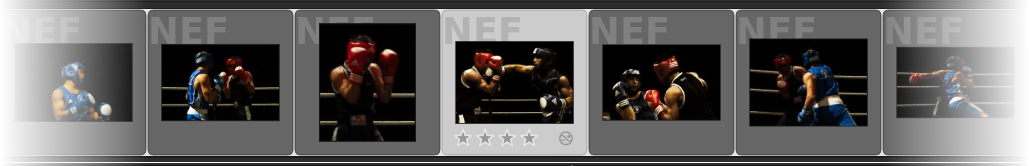
\includegraphics[height=1em]{filmstrip}} \\
    \end{tabularx}}

  \section{\LANGLighttable}

  \colorbox{keycol}{%
    \begin{tabularx}{\tabwidth}{k@{\tableseparator}X}
      0 -- 5 & \LANGRateImageWithStars\ \raisebox{-.15\height}{
\includegraphics[height=1em]{star_rating_panel}} \\
      f1 -- f5 & \LANGAssignColorLabel\ \raisebox{-.15\height}{
\includegraphics[height=1em]{color_labels_panel}} \\
      r & \LANGRejectImage \\
      \LANGDel & \LANGRemoveFromCollection \\
      \LANGCtrl-a & \LANGSelectAll \\
      \LANGCtrl-\LANGShift-a & \LANGSelectNone \\
      \LANGCtrl-i & \LANGInvertSelection \\
      \LANGAlt-1/2/3/4 & \LANGZoomMaxInOutMin \\
      \LANGCtrl-c & \LANGCopyHistoryStack \\
      \LANGCtrl-\LANGShift-c & \LANGCopyPartOfHistoryStack \\
      \LANGCtrl-v & \LANGPasteHistoryStack \\ 
      \LANGCtrl-\LANGShift-v & \LANGPastePartOfHistoryStack \\
      \LANGCtrl-d & \LANGDuplicateImage \\
      d & \LANGOpenInDarkroom \\
      z & \LANGZoomIntoImage \\
      \LANGCtrl-z & \LANGZoomAndShowFocusAreas \\
      \LANGCtrl-g & \LANGGroupImages \\
      \LANGCtrl-\LANGShift-g & \LANGUngroupImages \\
      \LANGCtrl-t & \LANGTag \\
      \LANGCtrl-k & \LANGJumpBackToPreviousCollection \\
      \LANGCtrl-\LANGShift-i & \LANGImportFolder \\
      \LANGCtrl-e & \LANGExport 
    \end{tabularx}}

  \section{\LANGSlideshow}

  \colorbox{keycol}{%
    \begin{tabularx}{\tabwidth}{k@{\tableseparator}X}
      \LANGLeftClick & \LANGNextImage \\
      \LANGRightClick & \LANGPreviousImage \\
      \LANGSpace & \LANGStartStop \\
      \LANGEsc & \LANGExitSlideshow \\
    \end{tabularx}}
  
  \bigskip

  \begin{center}
    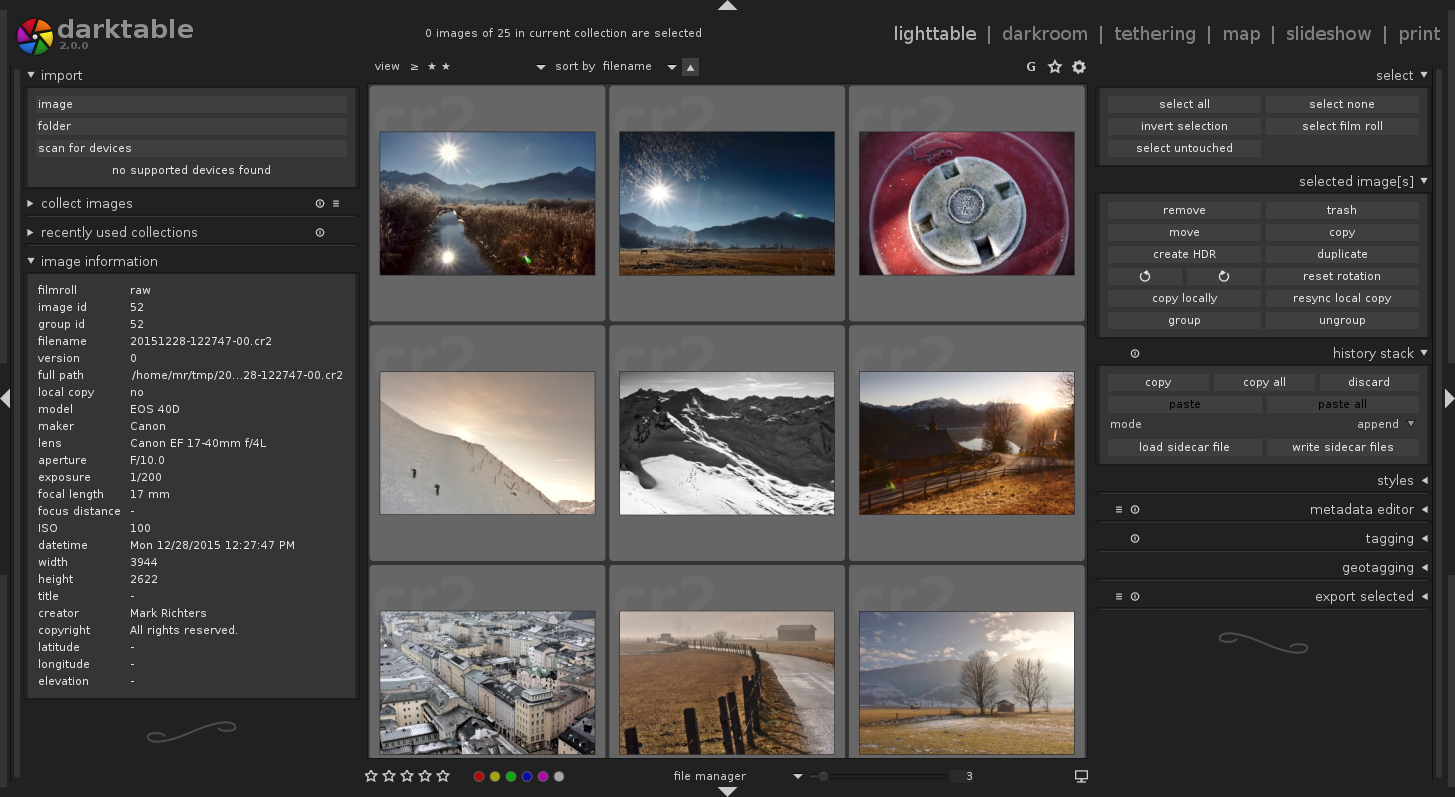
\includegraphics[height=5.5em]{lighttable_view2}
    \qquad
    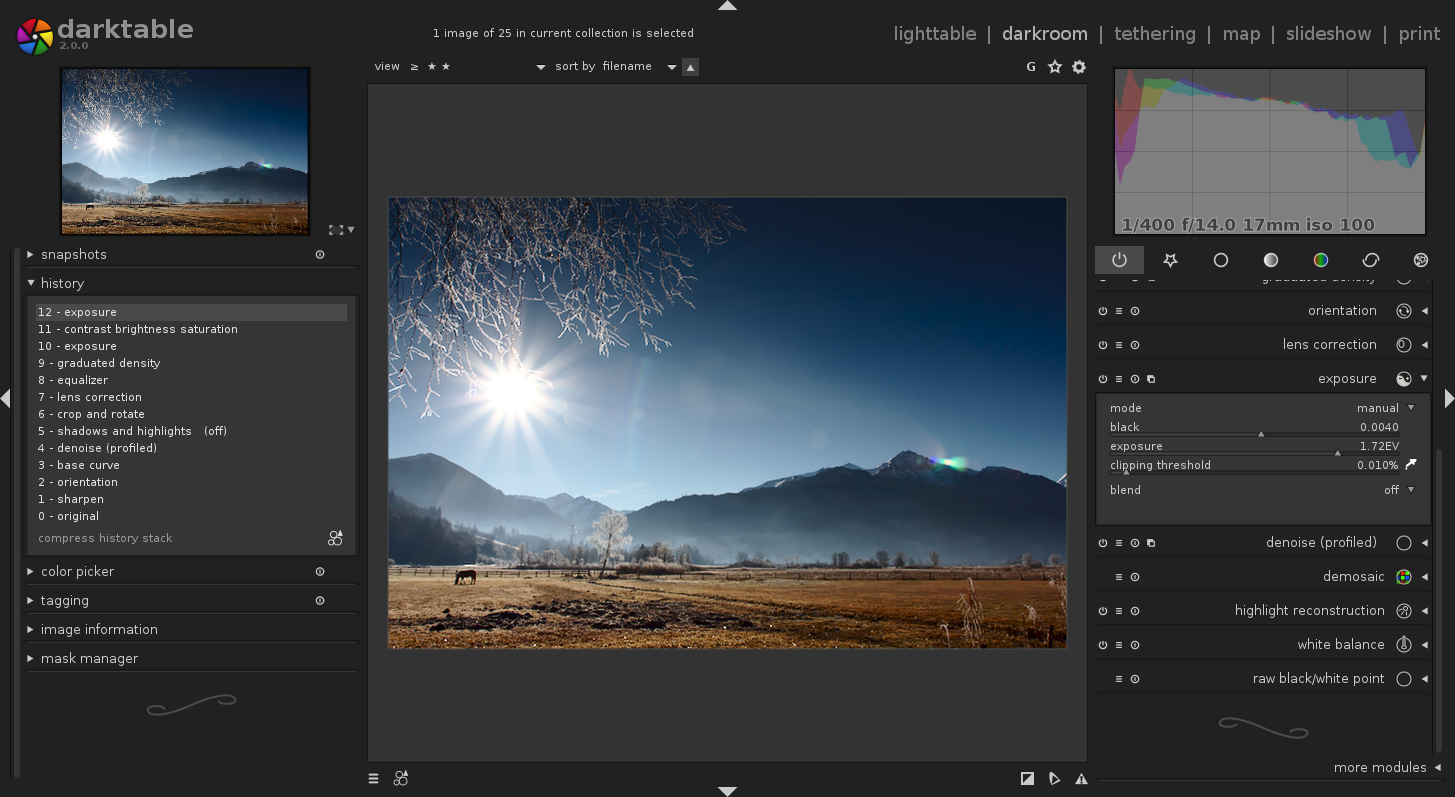
\includegraphics[height=5.5em]{darkroom_view2}
  \end{center}
  
  \section{\LANGDarkroom}

  \colorbox{keycol}{%
    \begin{tabularx}{\tabwidth}{k@{\tableseparator}X}
      c & \LANGCompressHistoryStack \\
      o & \LANGOverUnderexposed \\
      \LANGCtrl-e & \LANGExport \\
      \LANGSpace & \LANGNextImage \\
      \LANGBackspace & \LANGPreviousImage \\
      \mbox{[}/\mbox{\{}/\mbox{<} & \LANGDecreaseBrushSizeHardnessOpacity \\
      \mbox{]}/\mbox{\}}/\mbox{>} & \LANGIncreaseBrushSizeHardnessOpacity \\
      \LANGAlt-1/2/3 & \LANGZoomCloseUpFillFit \\
      \LANGCtrl-s & \LANGSoftproof \\
      \LANGCtrl-g & \LANGGamutCheck \\
      \LANGMiddleClick & \LANGZoomOneOneOrTwoOne \\
      \LANGMouseWheel & \LANGZoomBetweenOneOneAndFitToScreen \\
      \LANGCtrl-\LANGMouseWheel & \LANGZoomBetweenTwoOneAndOneOneZero \\
      \LANGShift-\LANGClick & \LANGExpandModuleKeepPreviousExpanded \\
    \end{tabularx}}
  
  \section{\LANGSliders}

  \colorbox{keycol}{%
    \begin{tabularx}{\tabwidth}{k@{\tableseparator}X}
      \LANGLeftClick\ + \LANGDrag & \LANGSetValue \\
      \LANGMouseWheel & \LANGSetValue \\
      \LANGRightClick & \LANGPopUpForMouseControlOrDirectValueEnter \\
      \LANGDoubleClick & \LANGResetToDefault \\
    \end{tabularx}}
  
  \small

  \section{\LANGBasicAndTone}

  \colorbox{keycol}{%
    \begin{tabularx}{\tabwidth}{clcl}
      
\includegraphics[height=1em]{colisa} & \LANGContrastBrightnessSaturation   & 
\includegraphics[height=1em]{relight} & \LANGFillLight \\
      
\includegraphics[height=1em]{shadhi} & \LANGShadowsAndHighlights           & 
\includegraphics[height=1em]{tonecurve} & \LANGToneCurve \\
      
\includegraphics[height=1em]{clipping} & \LANGCropAndRotate                & 
\includegraphics[height=1em]{zonesystem} & \LANGZoneSystem \\
      
\includegraphics[height=1em]{colorreconstruct} & \LANGColorReconstruction  & 
\includegraphics[height=1em]{levels} & \LANGLevels \\
      
\includegraphics[height=1em]{basecurve} & \LANGBaseCurve                   & 
\includegraphics[height=1em]{template} & \LANGLocalContrast \\
      
\includegraphics[height=1em]{flip} & \LANGOrientation                      & 
\includegraphics[height=1em]{template} & \LANGGlobalTonemap \\
      
\includegraphics[height=1em]{exposure} & \LANGExposure                     & 
\includegraphics[height=1em]{tonemap} & \LANGToneMapping \\
      
\includegraphics[height=1em]{demosaic} & \LANGDemosaic \\
      
\includegraphics[height=1em]{highlights} & \LANGHighlightReconstruction \\
      
\includegraphics[height=1em]{temperature} & \LANGWhiteBalance \\
      
\includegraphics[height=1em]{invert} & \LANGInvert \\
      
\includegraphics[height=1em]{template} & \LANGRawBlackWhitePoint \\
    \end{tabularx}}
  
  \section{\LANGColor}

  \colorbox{keycol}{%
    \begin{tabularx}{\tabwidth}{cl} 
      
\includegraphics[height=1em]{velvia} & \LANGVelvia \\
      
\includegraphics[height=1em]{channelmixer} & \LANGChannelMixer \\
      
\includegraphics[height=1em]{colorout} & \LANGOutputColorProfile \\
      
\includegraphics[height=1em]{template} & \LANGColorContrast \\
      
\includegraphics[height=1em]{colorcorrection} & \LANGColorCorrection \\
      
\includegraphics[height=1em]{monochrome} & \LANGMonochrome \\
      
\includegraphics[height=1em]{colorzones} & \LANGColorZones \\
      
\includegraphics[height=1em]{template} & \LANGColorBalance \\
      
\includegraphics[height=1em]{template} & \LANGVibrance \\
      
\includegraphics[height=1em]{colorin} & \LANGInputColorProfile \\
      
\includegraphics[height=1em]{profile_gamma} & \LANGUnbreakInputProfile \\
    \end{tabularx}}

  \section{\LANGCorrectionAndEffect}

  \colorbox{keycol}{%
    \begin{tabularx}{\tabwidth}{clcl}
      
\includegraphics[height=1em]{dither} & \LANGDithering                      & 
\includegraphics[height=1em]{watermark} & \LANGWatermark \\
      
\includegraphics[height=1em]{sharpen} & \LANGSharpen                       & 
\includegraphics[height=1em]{borders} & \LANGFraming \\
      
\includegraphics[height=1em]{atrous} & \LANGEqualizer                      & 
\includegraphics[height=1em]{splittoning} & \LANGSplitToning \\
      
\includegraphics[height=1em]{nlmeans} & \LANGDenoiseNonLocalMeans          & 
\includegraphics[height=1em]{vignette} & \LANGVignetting \\
      
\includegraphics[height=1em]{template} & \LANGDefringe                     & 
\includegraphics[height=1em]{soften} & \LANGSoften \\
      
\includegraphics[height=1em]{bilateral} & \LANGDenoiseBilateralFilter      & 
\includegraphics[height=1em]{grain} & \LANGGrain \\
      
\includegraphics[height=1em]{lens} & \LANGLensCorrection                   & \includegraphics[height=1em]{highpass} & \LANGHighpass \\
      \includegraphics[height=1em]{template} & \LANGScalePixels                  & \includegraphics[height=1em]{lowpass} & \LANGLowpass \\
      \includegraphics[height=1em]{template} & \LANGRotatePixels                 & \includegraphics[height=1em]{lowlight} & \LANGLowlightVision \\
      \includegraphics[height=1em]{spots} & \LANGSpotRemoval                     & \includegraphics[height=1em]{bloom} & \LANGBloom \\
      \includegraphics[height=1em]{template} & \LANGDenoiseProfiled              & \includegraphics[height=1em]{colormapping} & \LANGColorMapping \\
      \includegraphics[height=1em]{rawdenoise} & \LANGRawDenoise                 & \includegraphics[height=1em]{template} & \LANGColorize \\
      \includegraphics[height=1em]{hotpixels} & \LANGHotPixels                   & \includegraphics[height=1em]{graduatednd} & \LANGGraduated \\
      \includegraphics[height=1em]{cacorrect} & \LANGChromaticAberrations
    \end{tabularx}}

\end{multicols}
\end{document}

%%% Local Variables:
%%% TeX-master: "darktable-refcard-a4paper-english-dark-0.4pre"
%%% End:
